\documentclass[12pt, a4paper]{article}
\usepackage[english,russian]{babel}
\usepackage[warn]{mathtext}
\usepackage[T2A]{fontenc}
\usepackage[utf8]{inputenc}

\usepackage{color}
\usepackage{amssymb,amsmath}
\usepackage{graphicx}
\usepackage{multicol}

\textheight=24cm           % высота текста
\textwidth=16cm            % ширина текста
\oddsidemargin=0pt         % отступ от левого края
\topmargin=-1.5cm          % отступ от верхнего края
\parindent=24pt            % абзацный отступ
\parskip=0pt               % интервал между абзацами
\tolerance=2000            % терпимость к "жидким" строкам
\flushbottom               % выравнивание высоты страниц
%\def\baselinestretch{1.5} % печать с большим интервалом

%\title{}
%\author{\copyright~~С.А.~Назарова \thanks{e-mail:~sophia.nazarova@gmail.com}}
%\date{}

\begin{document}
\begin{figure}[h]

\begin{multicols}{2}
\hfill
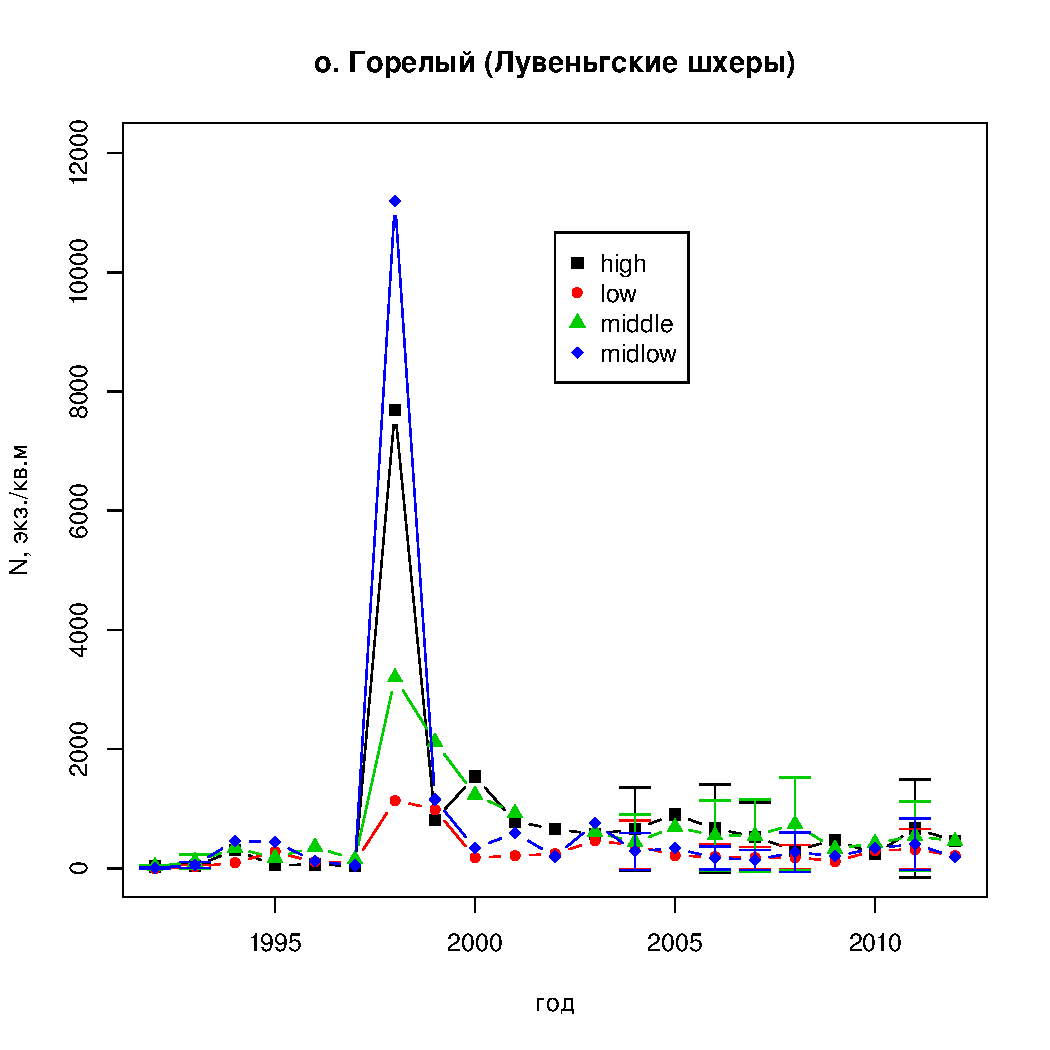
\includegraphics[width=65mm]{../White_Sea/Luvenga_Goreliy/N_dynamic.pdf}
\hfill
\includegraphics[width=65mm]{../White_Sea//Luvenga_II_razrez/N_dynamic.pdf}
\end{multicols}

%\smallskip


\begin{multicols}{2}
\hfill
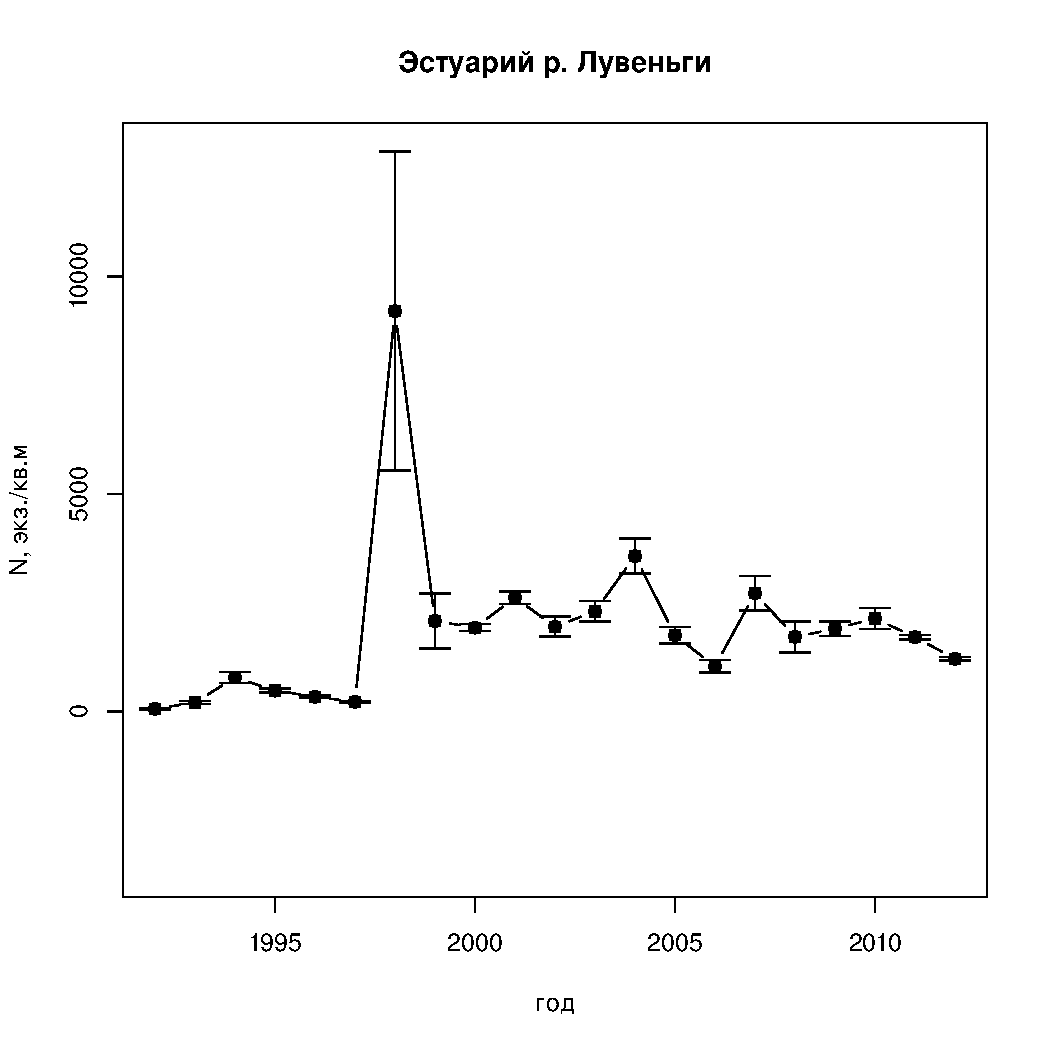
\includegraphics[width=65mm]{../White_Sea/Estuatiy_Luvenga/N_dynamic.pdf}
\hfill
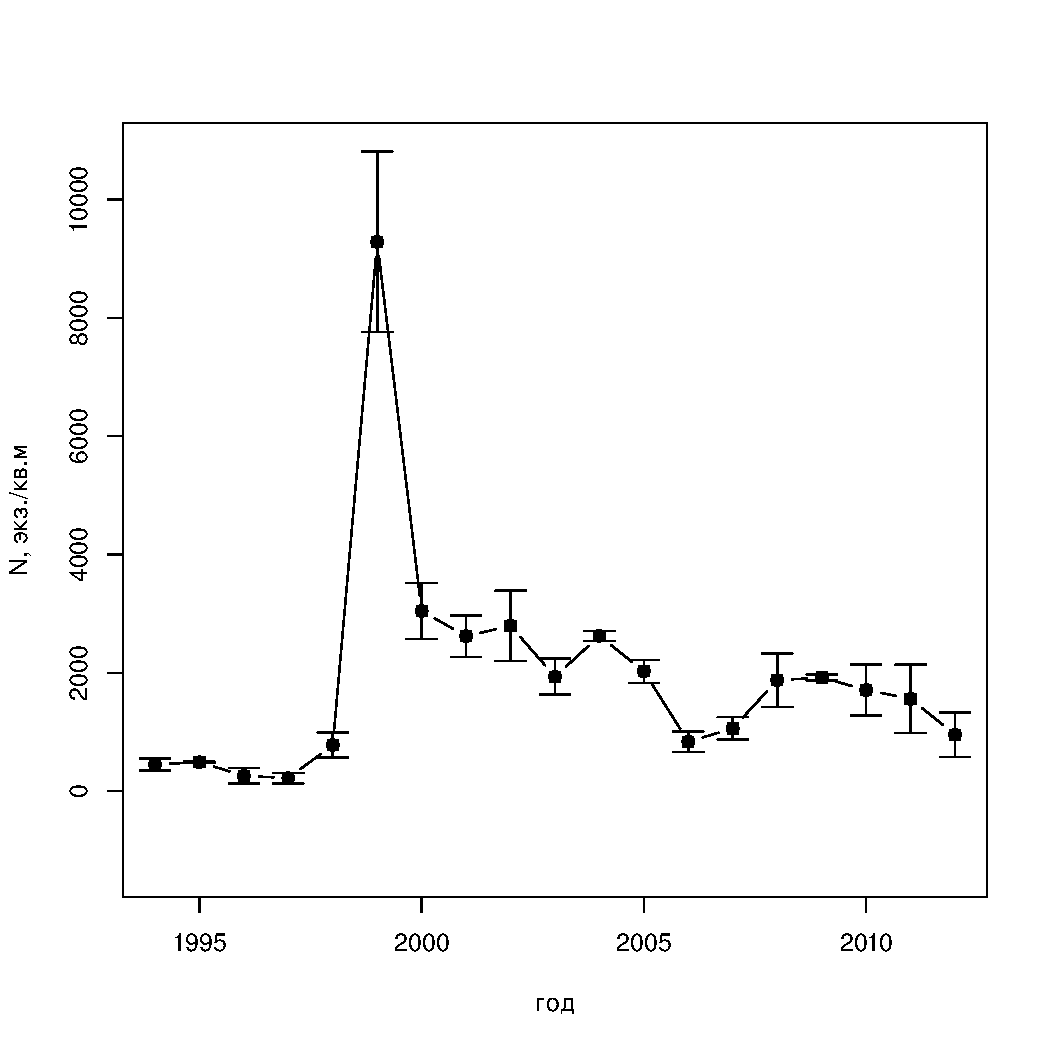
\includegraphics[width=65mm]{../White_Sea/Ryashkov_ZRS/N_dynamic.pdf}
\end{multicols}

%\smallskip

\begin{multicols}{2}
\hfill
\includegraphics[width=65mm]{../White_Sea/Ryashkov_YuG/N_dynamic.pdf}
\hfill
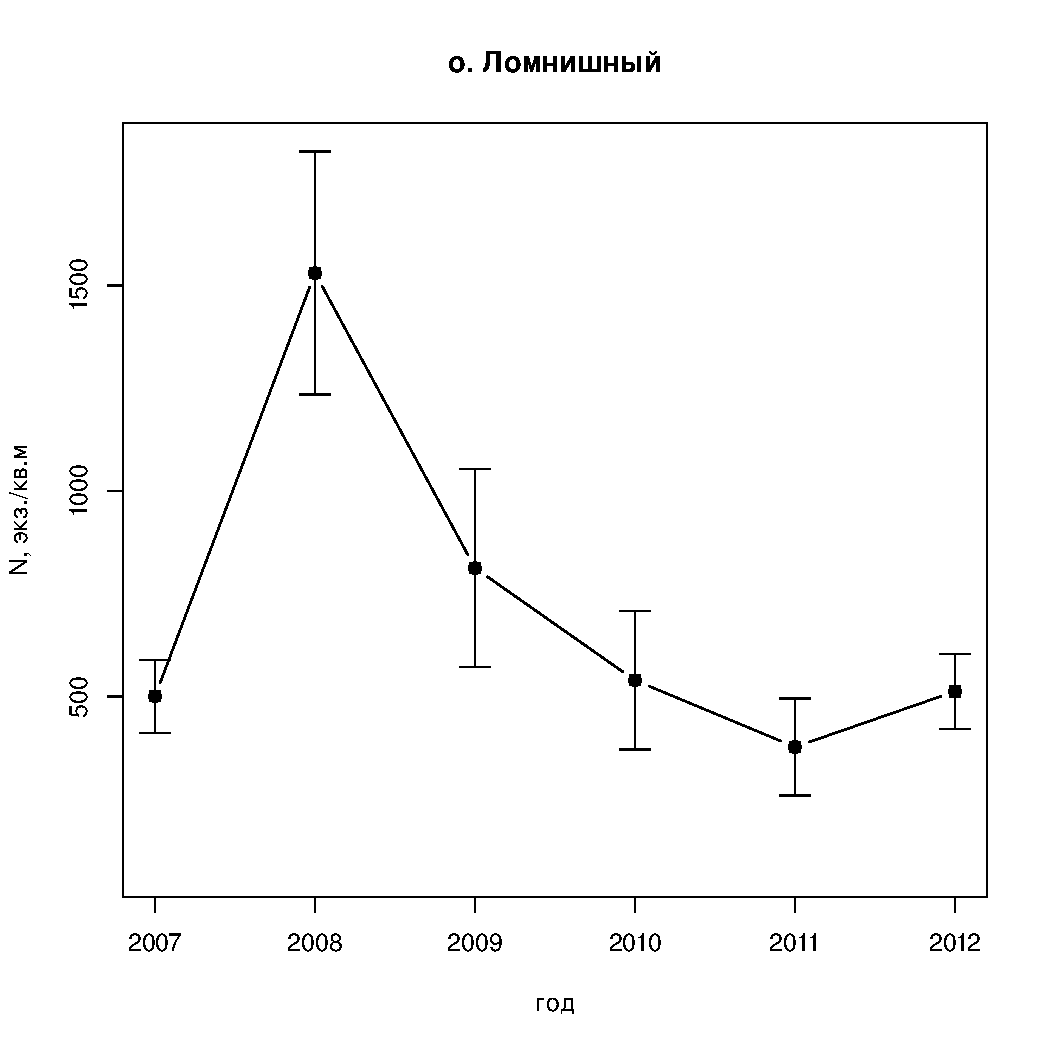
\includegraphics[width=65mm]{../White_Sea/Lomnishniy/N_dynamic.pdf}
\end{multicols}

%\smallskip


\caption{Динамика плотности поселений {\it Macoma balthica} в вершине Кандалакшского залива}
\label{ris:dynamic_Kandalaksha_all}
\end{figure}


\end{document}
